\section*{Chapter 13}

\subsection*{Problem 13.1}
Develop expressions for the mole fractions of reacting species as
functions of the reaction coordinate for:

\begin{abcls}
\item A system containing 2~\unit{\mole} \(\ce{NH3}\) and
  5~\unit{\mole} \(\ce{O2}\) and undergoing the reaction:
  \begin{equation*}
    \ce{4NH3(g) + 5O2(g) -> 4NO(g) + 6H2O(g)}
  \end{equation*}
\item A system initially containing 3~\unit{\mole} \(\ce{H2S}\) and
  5~\unit{\mole} \(\ce{O2}\) and undergoing the reaction:
  \begin{equation*}
    \ce{2H2S(g) + 3O2(g) -> 2H2O(g) + 2SO2(g)}
  \end{equation*}
\item A system containing 3~\unit{\mole} \(\ce{NO2}\),
  4~\unit{\mole} \(\ce{NH3}\), and 1~\unit{\mole} \(\ce{N2}\) and
  undergoing the reaction:
  \begin{equation*}
    \ce{6NO2(g) + 8NH3(g) -> 7N2(g) + 12H2O(g)}
  \end{equation*}
\end{abcls}

\begin{solution}
  The solution here is to substitute into Eq.~(\ref{eq:yeq})
  \begin{equation}
    \label{eq:yeq}
    y_i = \frac{n_{io} + v_{i}\varepsilon}{n_0 + v\varepsilon} \tag{13.5}
  \end{equation}
  \begin{abcls}
  \item
    \begin{empheq}[box=\widefbox]{gather*}
      y_{\ce{NH3}} = \frac{2 - 4\varepsilon}{7 + \varepsilon} \\
      y_{\ce{O2}} = \frac{5 - 5\varepsilon}{7 + \varepsilon}
    \end{empheq}
  \item
    \begin{empheq}[box=\widefbox]{gather*}
      y_{\ce{H2S}} = \frac{3 - 2\varepsilon}{8 - \varepsilon} \\
      y_{\ce{O2}} = \frac{5 - 3\varepsilon}{8 - \varepsilon}
    \end{empheq}
  \item
    \begin{empheq}[box=\widefbox]{gather*}
      y_{\ce{NO2}} = \frac{3 - 6\varepsilon}{8 + 5\varepsilon} \\
      y_{\ce{NH3}} = \frac{4 - 8\varepsilon}{8 + 5\varepsilon} \\
      y_{\ce{N2}} = \frac{1 + 7\varepsilon}{8 + 5\varepsilon}
    \end{empheq}
  \end{abcls}
\end{solution}

\subsection*{Problem 13.2}
A system initially containing 2~\unit{\mole} \(\ce{C2H4}\) and
3~\unit{\mole} \(\ce{O2}\) undergoes the reactions:
\begin{gather*}
  \ce{C2H4(g) + \frac{1}{2}O2(g) -> ((CH2)2)O(g)} \\
  \ce{C2H4(g) + 3O2(g) -> 2CO2(g) + 2H2O(g)}
\end{gather*}
Develop expressions for the mole fractions of the reacting species as
functions of the reaction coordinates for the two reactions.

\begin{solution}
  The two chemical reactions need to be added and the same solution
  in Problem~13.1 is to be used.
  \begin{gather*}
    \ce{2C2H4(g) + 3.5O2(g) -> 2CO2(g) + 2H2O(g) + ((CH2)2)O(g)}
  \end{gather*}
  \begin{empheq}[box=\widefbox]{gather*}
    y_{\ce{C2H4}} = \frac{2 - 2\varepsilon}{5} \\
    y_{\ce{O2}} = \frac{3 - 3.5\varepsilon}{5}
  \end{empheq}
\end{solution}

\subsection*{Problem 13.3}
A system formed initially of 2~\unit{\mole} \(\ce{CO2}\),
5~\unit{\mole} \(\ce{H2}\), and 1~\unit{\mole} \(\ce{CO}\) undergoes
the reactions:
\begin{gather*}
  \ce{CO2(g) + 3H2(g) -> CH3OH(g) + H2O(g)} \\
  \ce{CO2(g) + H2(g) -> CO(g) + H2O(g)}
\end{gather*}
Develop expressions for the mole fractions of the reacting species as
functions of the reaction coordinates for the two reactions.

\begin{solution}
  Similar to the previous problem.
  \begin{gather*}
    \ce{2CO2(g) + 4H2(g) -> CH3OH(g) + 2H2O(g) + CO(g)}
  \end{gather*}
  \begin{empheq}[box=\widefbox]{gather*}
    y_{\ce{CO2}} = \frac{2 - 2\varepsilon}{8 - 2\varepsilon} \\
    y_{\ce{H2}} = \frac{5 - 4\varepsilon}{8 - 2\varepsilon} \\
    y_{\ce{CO}} = \frac{1 + \varepsilon}{8 - 2\varepsilon}
  \end{empheq}
\end{solution}

\subsection*{Problem 13.4}
Consider the water-gas-shift reaction:
\begin{equation*}
  \ce{H2(g) + CO2(g) -> H2O(g) + CO(g)}
\end{equation*}
At high temperatures and low to moderate pressures the reacting
species form an ideal-gas mixture. By Eq.~(11.27):
\begin{equation*}
  G = \sum_{i}^{~}y_iG_i + RT\sum_{i}^{~}y_i\ln y_i
\end{equation*}
When the Gibbs energies of the elements in their standard states are
set equal to zero, \(G_i = \Delta G_{f_i}^\circ\), for each species, and then:
\begin{equation}
  \label{eq:13.4G}
  G = \sum_{i}^{~}y_i\Delta G_{f_i}^\circ + RT\sum_{i}^{~}y_i \ln y_i \tag{A}
\end{equation}
At the beginning of Sec. 13.2 we noted that Eq.~(14.68) is a
criterion of equilibrium. Applied to the water-gas-shift reaction
with the understanding that \(T\) and \(P\) are constant, this equation becomes:
\begin{equation*}
  dG' = d(nG) = ndG + Gdn = 0 \qquad n\frac{dG}{d\varepsilon} +
  G\frac{dn}{d\varepsilon} = 0
\end{equation*}
Here, however, \(dn/d\varepsilon = 0\). The equilibrium criterion
therefore becomes:
\begin{equation}
  \label{eq:13.4dG}
  \frac{dG}{d\varepsilon} = 0 \tag{B}
\end{equation}
Once the \(y_i\) are eliminated in favor of \(\varepsilon\),
Eq.~(\ref{eq:13.4G}) relates \(G\) to \(\varepsilon\). Data for
\(\Delta G_{f_i}^\circ\) for the compounds of interest are givent
with Ex. 13.13. For a temperature of 1000~\unit{\kelvin} (the
reaction is unaffected by \(P\)) and for a feed of 1~\unit{\mole}
\(\ce{H2}\) and 1~\unit{\mole} \(\ce{CO2}\):
\begin{abcls}
\item Determine the equilibrium value of \(\varepsilon\) by
  application of Eq.~(\ref{eq:13.4dG}).
\item Plot \(G\) vs. \(\varepsilon\), indicating the location of
  the equilibrium value of \(\varepsilon\) determined in (a).
\end{abcls}

\begin{solution}
  \begin{enumerate}[label=(\alph*)]
    \item Solving for $\varepsilon$:
      \begin{gather*}
        y_{\ce{H2}} = y_{\ce{CO2}} = \frac{1 - \varepsilon}{2} \\
        y_{\ce{H2O}} = y_{\ce{CO}} = \frac{\varepsilon}{2} \\
        \intertext{From Eq.~(\ref{eq:13.4G})---the values of
          \(\Delta G_{f_i}^\circ\) in \unit{\joule\per\mole} are given
        in Example~13.13:}
        \begin{split}
          G = \left(\frac{1-\varepsilon}{2}\right)(-395790) +
          \left(\frac{\varepsilon}{2}\right)(-200240 - 192420) + \\
          R(1000)\left[2\left(\frac{1-\varepsilon}{2}\right)
            \ln\left(\frac{1-\varepsilon}{2}\right) +
            2\left(\frac{\varepsilon}{2}\right) \ln
          \left(\frac{\varepsilon}{2}\right)\right]
        \end{split}
        \intertext{Differentiate with respect to \(\varepsilon\) and
        solve for the root as in Eq.~(\ref{eq:13.4dG}):}
        \boxed{\varepsilon = 0.452}
      \end{gather*}
    \item See Figure~\ref{fig:13.4}
  \end{enumerate}
\end{solution}

\begin{figure}[H]
  \centering
  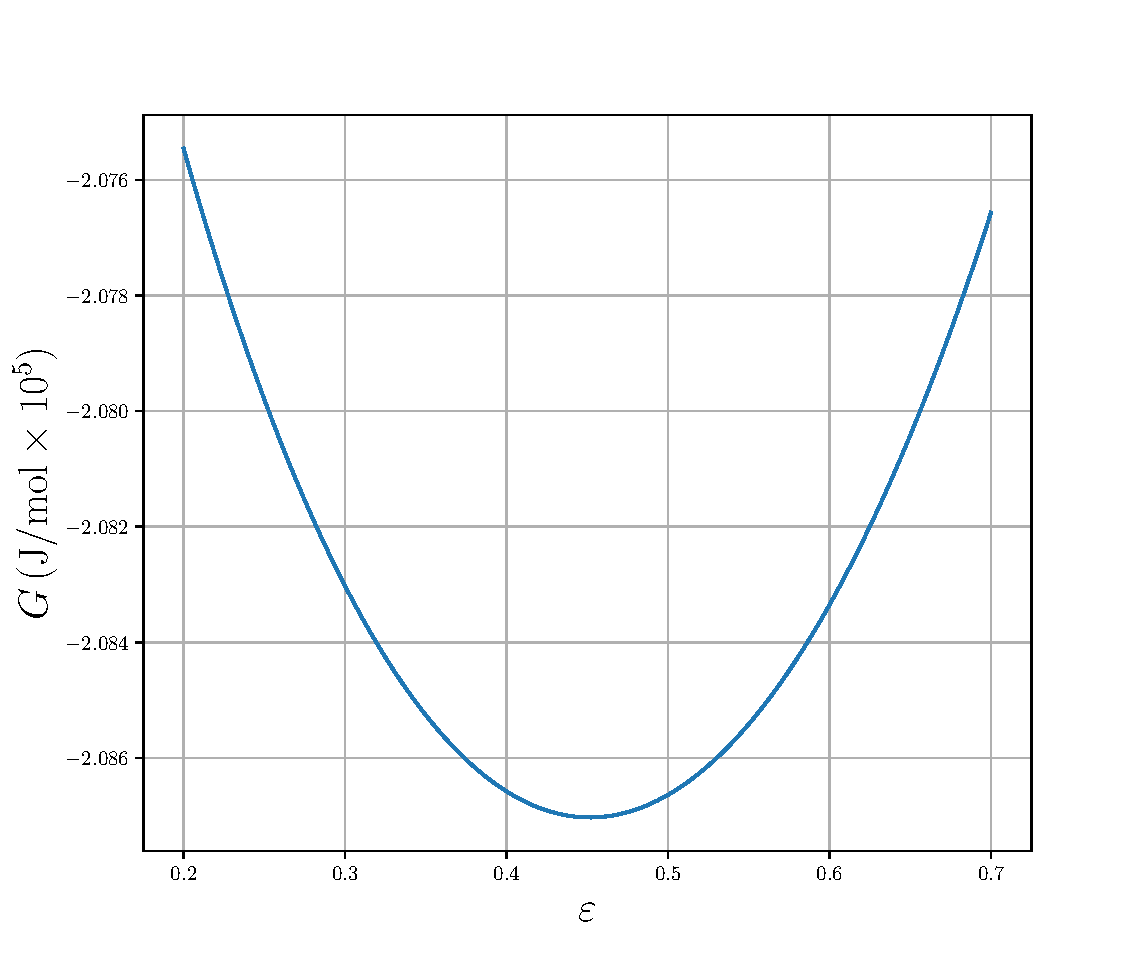
\includegraphics[scale=0.5]{assets/13_4.pdf}
  \caption{The graph of $G$ with respect to $\varepsilon$ for the
  system described in 13.4}
  \label{fig:13.4}
\end{figure}

\subsection*{Problem 13.5}
Rework Pb. 13.4 for a temperature of:
\begin{enumerate}[label=(\alph*)]
  \item \(1100~\unit{\kelvin}\);
  \item \(1200~\unit{\kelvin}\);
  \item \(1300~\unit{\kelvin}\).
\end{enumerate}

\begin{solution}
  Refer to Pb. 13.4 for the solution.
  The plots of (a), (b), and (c) are shown in Figure~\ref{fig:13.5}
  \begin{enumerate}[label=(\alph*)]
    \item \(\boxed{\varepsilon=0.456\)}
    \item \(\boxed{\varepsilon=0.460\)}
    \item \(\boxed{\varepsilon=0.463\)}
  \end{enumerate}
\end{solution}

\begin{figure}[H]
  \centering
  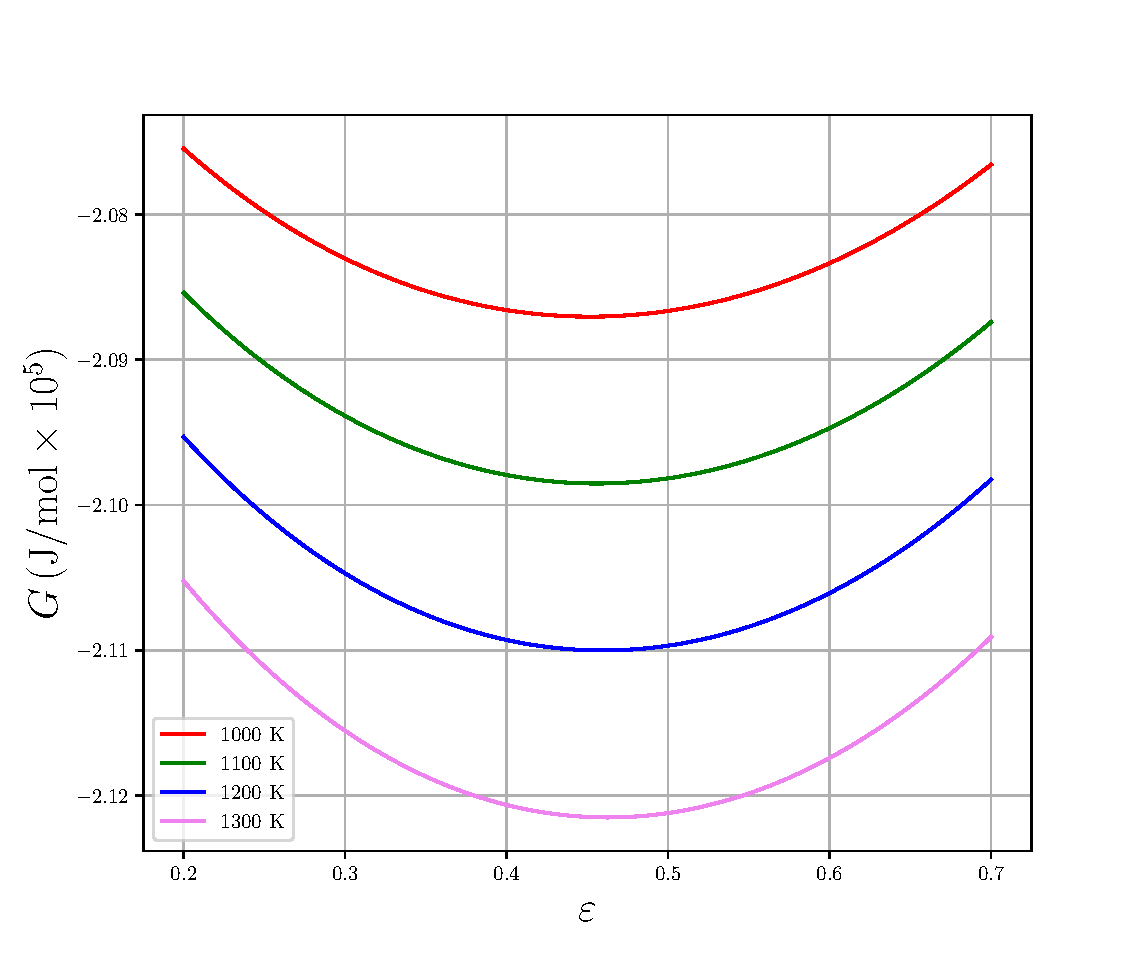
\includegraphics[scale=0.5]{assets/13_5.pdf}
  \caption{The graph of \(G\) with respect to \(\varepsilon\) for the
  systems described in 13.5}
  \label{fig:13.5}
\end{figure}
